% ---------------------------------------------------------------
% Generated by FlowTikZ (flowcharts and data charts to LaTeX)
% Every coordinate below is derived from the editor diagram model.
% Safe to edit by hand, but regenerating will overwrite changes.
% ---------------------------------------------------------------

\documentclass[border=8pt]{standalone}
\usepackage[T1]{fontenc}
\usepackage[utf8]{inputenc}
\usepackage{amsmath}
\usepackage{amssymb}
\usepackage{xcolor}
\usepackage{tikz}
\usepackage[american]{circuitikz}

% ---- Colour definitions ----
\definecolor{fc12161C}{HTML}{12161C}
\definecolor{fc1F2933}{HTML}{1F2933}
\definecolor{fc2563EB}{HTML}{2563EB}
\definecolor{fc64748B}{HTML}{64748B}
\definecolor{fcDC2626}{HTML}{DC2626}

% ---- Style definitions ----
\tikzset{
  fcnode/.style={
    draw, inner sep=0pt, outer sep=0pt, align=center,
    line join=round, line cap=butt
  },
  fcpath/.style={line join=round, line cap=butt},
  fcedge/.style={line join=round, line cap=butt},
  fclabel/.style={inner sep=1.4pt, outer sep=0pt, align=center},
}
\tikzset{fcformula/.style={inner sep=0pt, outer sep=0pt}}
\tikzset{fccircuit/.style={line join=round, line cap=butt,
  /tikz/circuitikz/bipoles/thickness=1, /tikz/circuitikz/tripoles/thickness=1}}

\begin{document}
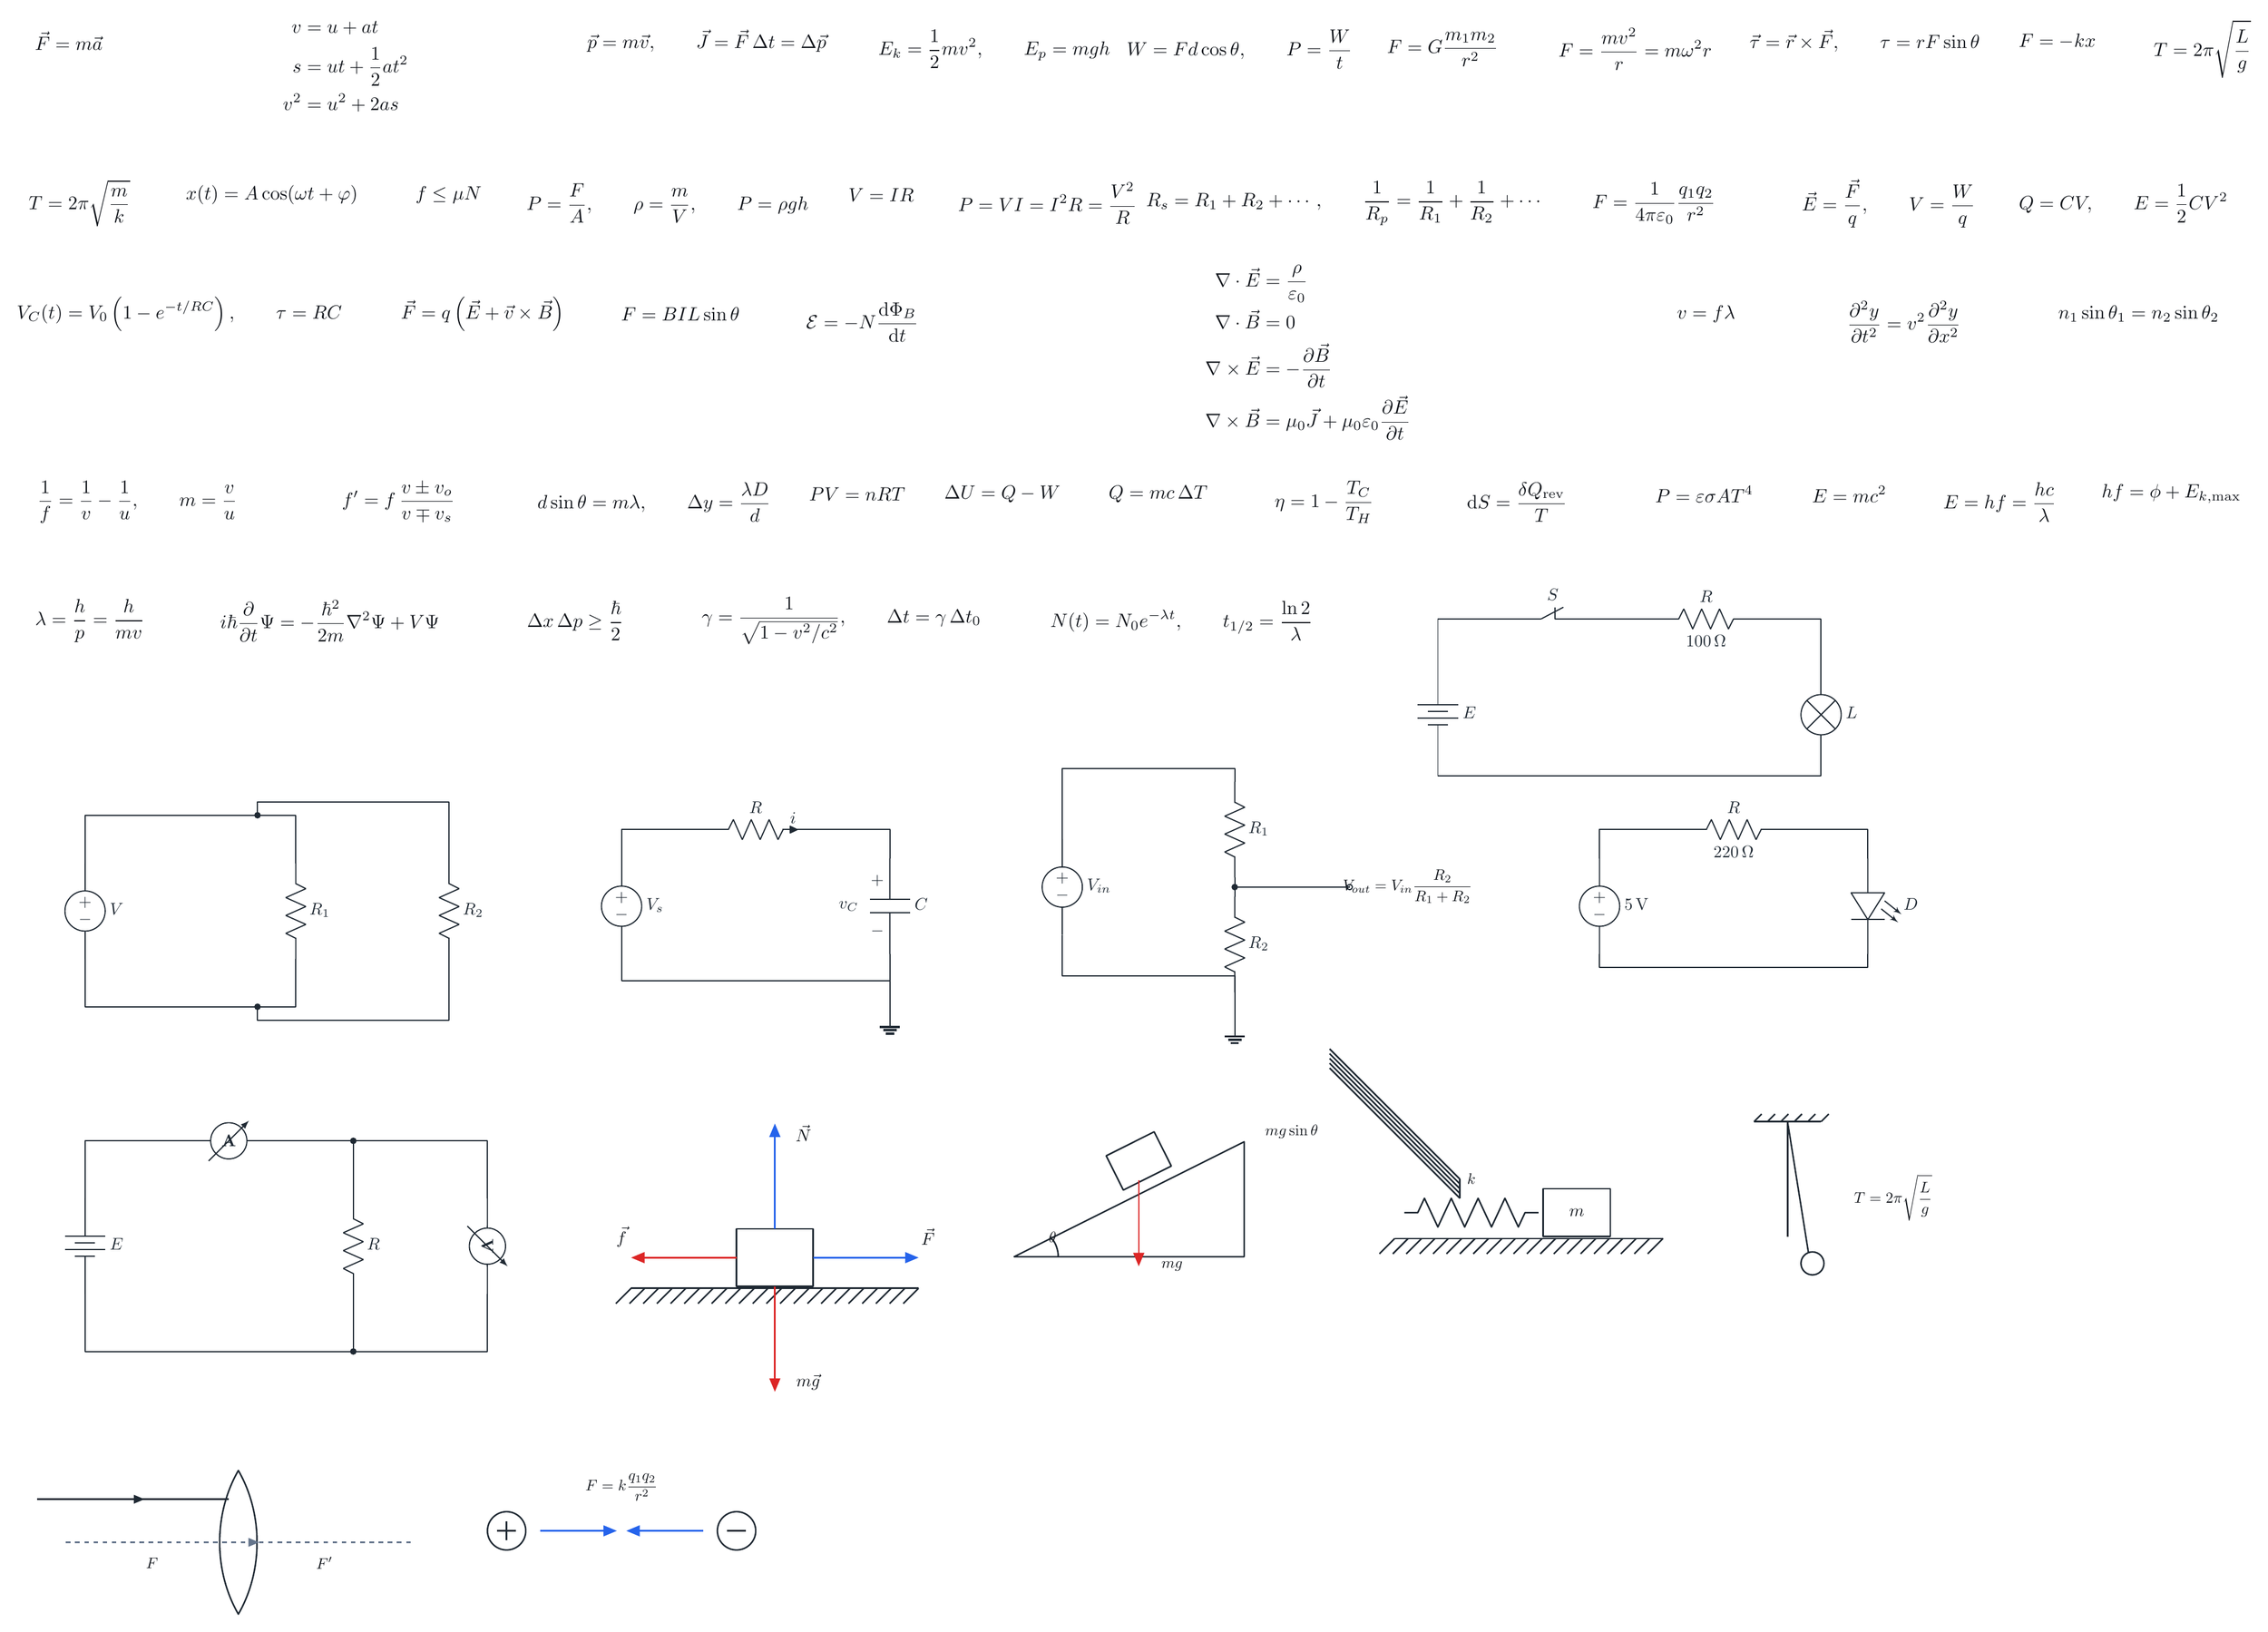
\begin{tikzpicture}[x=1cm, y=1cm]
  % ---- Nodes ----
  % g1 - Formula "\vec{F}=m\vec{a}"
  \node[fcformula, scale=1.138, text=fc12161C]
        (g1) at (2.66,-2.27) {$\displaystyle \vec{F}=m\vec{a}$};
  % g2 - Formula "\begin{aligned} v&=u+at \\ s&=ut+\frac{1}{2}at^{"
  \node[fcformula, scale=1.138, text=fc12161C]
        (g2) at (8.44,-2.81) {$\displaystyle \begin{aligned} v&=u+at \\ s&=ut+\frac{1}{2}at^{2} \\ v^{2}&=u^{2}+2as \end{aligned}$};
  % g3 - Formula "\vec{p}=m\vec{v},\qquad \vec{J}=\vec{F}\,\Delta "
  \node[fcformula, scale=1.138, text=fc12161C]
        (g3) at (15.98,-2.27) {$\displaystyle \vec{p}=m\vec{v},\qquad \vec{J}=\vec{F}\,\Delta t=\Delta\vec{p}$};
  % g4 - Formula "E_{k}=\frac{1}{2}mv^{2},\qquad E_{p}=mgh"
  \node[fcformula, scale=1.138, text=fc12161C]
        (g4) at (21.98,-2.44) {$\displaystyle E_{k}=\frac{1}{2}mv^{2},\qquad E_{p}=mgh$};
  % g5 - Formula "W=Fd\cos\theta,\qquad P=\frac{W}{t}"
  \node[fcformula, scale=1.138, text=fc12161C]
        (g5) at (27.1,-2.44) {$\displaystyle W=Fd\cos\theta,\qquad P=\frac{W}{t}$};
  % g6 - Formula "F=G\frac{m_{1}m_{2}}{r^{2}}"
  \node[fcformula, scale=1.138, text=fc12161C]
        (g6) at (31.34,-2.44) {$\displaystyle F=G\frac{m_{1}m_{2}}{r^{2}}$};
  % g7 - Formula "F=\frac{mv^{2}}{r}=m\omega^{2}r"
  \node[fcformula, scale=1.138, text=fc12161C]
        (g7) at (35.36,-2.44) {$\displaystyle F=\frac{mv^{2}}{r}=m\omega^{2}r$};
  % g8 - Formula "\vec{\tau}=\vec{r}\times\vec{F},\qquad \tau=rF\s"
  \node[fcformula, scale=1.138, text=fc12161C]
        (g8) at (40.15,-2.27) {$\displaystyle \vec{\tau}=\vec{r}\times\vec{F},\qquad \tau=rF\sin\theta$};
  % g9 - Formula "F=-kx"
  \node[fcformula, scale=1.138, text=fc12161C] (g9) at (44.17,-2.27) {$\displaystyle F=-kx$};
  % g10 - Formula "T=2\pi\sqrt{\frac{L}{g}}"
  \node[fcformula, scale=1.138, text=fc12161C]
        (g10) at (47.2,-2.44) {$\displaystyle T=2\pi\sqrt{\frac{L}{g}}$};
  % g11 - Formula "T=2\pi\sqrt{\frac{m}{k}}"
  \node[fcformula, scale=1.138, text=fc12161C]
        (g11) at (2.88,-5.66) {$\displaystyle T=2\pi\sqrt{\frac{m}{k}}$};
  % g12 - Formula "x(t)=A\cos(\omega t+\varphi)"
  \node[fcformula, scale=1.138, text=fc12161C]
        (g12) at (6.9,-5.49) {$\displaystyle x(t)=A\cos(\omega t+\varphi)$};
  % g13 - Formula "f\leq\mu N"
  \node[fcformula, scale=1.138, text=fc12161C]
        (g13) at (10.59,-5.49) {$\displaystyle f\leq\mu N$};
  % g14 - Formula "P=\frac{F}{A},\qquad \rho=\frac{m}{V},\qquad P=\"
  \node[fcformula, scale=1.138, text=fc12161C]
        (g14) at (15.16,-5.66) {$\displaystyle P=\frac{F}{A},\qquad \rho=\frac{m}{V},\qquad P=\rho gh$};
  % g15 - Formula "V=IR"
  \node[fcformula, scale=1.138, text=fc12161C] (g15) at (19.62,-5.49) {$\displaystyle V=IR$};
  % g16 - Formula "P=VI=I^{2}R=\frac{V^{2}}{R}"
  \node[fcformula, scale=1.138, text=fc12161C]
        (g16) at (23.09,-5.66) {$\displaystyle P=VI=I^{2}R=\frac{V^{2}}{R}$};
  % g17 - Formula "R_{s}=R_{1}+R_{2}+\cdots,\qquad \frac{1}{R_{p}}="
  \node[fcformula, scale=1.138, text=fc12161C]
        (g17) at (29.31,-5.66) {$\displaystyle R_{s}=R_{1}+R_{2}+\cdots,\qquad \frac{1}{R_{p}}=\frac{1}{R_{1}}+\frac{1}{R_{2}}+\cdots$};
  % g18 - Formula "F=\frac{1}{4\pi\varepsilon_{0}}\frac{q_{1}q_{2}}"
  \node[fcformula, scale=1.138, text=fc12161C]
        (g18) at (35.75,-5.66) {$\displaystyle F=\frac{1}{4\pi\varepsilon_{0}}\frac{q_{1}q_{2}}{r^{2}}$};
  % g19 - Formula "\vec{E}=\frac{\vec{F}}{q},\qquad V=\frac{W}{q}"
  \node[fcformula, scale=1.138, text=fc12161C]
        (g19) at (40.65,-5.66) {$\displaystyle \vec{E}=\frac{\vec{F}}{q},\qquad V=\frac{W}{q}$};
  % g20 - Formula "Q=CV,\qquad E=\frac{1}{2}CV^{2}"
  \node[fcformula, scale=1.138, text=fc12161C]
        (g20) at (45.55,-5.66) {$\displaystyle Q=CV,\qquad E=\frac{1}{2}CV^{2}$};
  % g21 - Formula "V_{C}(t)=V_{0}\left(1-e^{-t/RC}\right),\qquad \t"
  \node[fcformula, scale=1.138, text=fc12161C]
        (g21) at (4.97,-7.97) {$\displaystyle V_{C}(t)=V_{0}\left(1-e^{-t/RC}\right),\qquad \tau=RC$};
  % g22 - Formula "\vec{F}=q\left(\vec{E}+\vec{v}\times\vec{B}\righ"
  \node[fcformula, scale=1.138, text=fc12161C]
        (g22) at (11.3,-7.97) {$\displaystyle \vec{F}=q\left(\vec{E}+\vec{v}\times\vec{B}\right)$};
  % g23 - Formula "F=BIL\sin\theta"
  \node[fcformula, scale=1.138, text=fc12161C]
        (g23) at (15.43,-7.97) {$\displaystyle F=BIL\sin\theta$};
  % g24 - Formula "\mathcal{E}=-N\frac{\mathrm{d}\Phi_{B}}{\mathrm{"
  \node[fcformula, scale=1.138, text=fc12161C]
        (g24) at (19.23,-8.14) {$\displaystyle \mathcal{E}=-N\frac{\mathrm{d}\Phi_{B}}{\mathrm{d}t}$};
  % g25 - Formula "\begin{aligned} \nabla\cdot\vec{E}&=\frac{\rho}{"
  \node[fcformula, scale=1.138, text=fc12161C]
        (g25) at (28.53,-8.78) {$\displaystyle \begin{aligned} \nabla\cdot\vec{E}&=\frac{\rho}{\varepsilon_{0}} \\ \nabla\cdot\vec{B}&=0 \\ \nabla\times\vec{E}&=-\frac{\partial\vec{B}}{\partial t} \\ \nabla\times\vec{B}&=\mu_{0}\vec{J}+\mu_{0}\varepsilon_{0}\frac{\partial\vec{E}}{\partial t} \end{aligned}$};
  % g26 - Formula "v=f\lambda"
  \node[fcformula, scale=1.138, text=fc12161C]
        (g26) at (36.84,-7.97) {$\displaystyle v=f\lambda$};
  % g27 - Formula "\frac{\partial^{2}y}{\partial t^{2}}=v^{2}\frac{"
  \node[fcformula, scale=1.138, text=fc12161C]
        (g27) at (40.97,-8.14) {$\displaystyle \frac{\partial^{2}y}{\partial t^{2}}=v^{2}\frac{\partial^{2}y}{\partial x^{2}}$};
  % g28 - Formula "n_{1}\sin\theta_{1}=n_{2}\sin\theta_{2}"
  \node[fcformula, scale=1.138, text=fc12161C]
        (g28) at (45.87,-7.97) {$\displaystyle n_{1}\sin\theta_{1}=n_{2}\sin\theta_{2}$};
  % g29 - Formula "\frac{1}{f}=\frac{1}{v}-\frac{1}{u},\qquad m=\fr"
  \node[fcformula, scale=1.138, text=fc12161C]
        (g29) at (4.09,-11.9) {$\displaystyle \frac{1}{f}=\frac{1}{v}-\frac{1}{u},\qquad m=\frac{v}{u}$};
  % g30 - Formula "f'=f\,\frac{v\pm v_{o}}{v\mp v_{s}}"
  \node[fcformula, scale=1.138, text=fc12161C]
        (g30) at (9.54,-11.9) {$\displaystyle f'=f\,\frac{v\pm v_{o}}{v\mp v_{s}}$};
  % g31 - Formula "d\sin\theta=m\lambda,\qquad \Delta y=\frac{\lamb"
  \node[fcformula, scale=1.138, text=fc12161C]
        (g31) at (14.88,-11.9) {$\displaystyle d\sin\theta=m\lambda,\qquad \Delta y=\frac{\lambda D}{d}$};
  % g32 - Formula "PV=nRT"
  \node[fcformula, scale=1.138, text=fc12161C]
        (g32) at (19.12,-11.73) {$\displaystyle PV=nRT$};
  % g33 - Formula "\Delta U=Q-W"
  \node[fcformula, scale=1.138, text=fc12161C]
        (g33) at (22.15,-11.73) {$\displaystyle \Delta U=Q-W$};
  % g34 - Formula "Q=mc\,\Delta T"
  \node[fcformula, scale=1.138, text=fc12161C]
        (g34) at (25.4,-11.73) {$\displaystyle Q=mc\,\Delta T$};
  % g35 - Formula "\eta=1-\frac{T_{C}}{T_{H}}"
  \node[fcformula, scale=1.138, text=fc12161C]
        (g35) at (28.87,-11.9) {$\displaystyle \eta=1-\frac{T_{C}}{T_{H}}$};
  % g36 - Formula "\mathrm{d}S=\frac{\delta Q_{\text{rev}}}{T}"
  \node[fcformula, scale=1.138, text=fc12161C]
        (g36) at (32.89,-11.9) {$\displaystyle \mathrm{d}S=\frac{\delta Q_{\text{rev}}}{T}$};
  % g37 - Formula "P=\varepsilon\sigma AT^{4}"
  \node[fcformula, scale=1.138, text=fc12161C]
        (g37) at (36.8,-11.73) {$\displaystyle P=\varepsilon\sigma AT^{4}$};
  % g38 - Formula "E=mc^{2}"
  \node[fcformula, scale=1.138, text=fc12161C]
        (g38) at (39.83,-11.73) {$\displaystyle E=mc^{2}$};
  % g39 - Formula "E=hf=\frac{hc}{\lambda}"
  \node[fcformula, scale=1.138, text=fc12161C]
        (g39) at (42.97,-11.9) {$\displaystyle E=hf=\frac{hc}{\lambda}$};
  % g40 - Formula "hf=\phi+E_{k,\max}"
  \node[fcformula, scale=1.138, text=fc12161C]
        (g40) at (46.55,-11.73) {$\displaystyle hf=\phi+E_{k,\max}$};
  % g41 - Formula "\lambda=\frac{h}{p}=\frac{h}{mv}"
  \node[fcformula, scale=1.138, text=fc12161C]
        (g41) at (3.1,-14.38) {$\displaystyle \lambda=\frac{h}{p}=\frac{h}{mv}$};
  % g42 - Formula "i\hbar\frac{\partial}{\partial t}\Psi=-\frac{\hb"
  \node[fcformula, scale=1.138, text=fc12161C]
        (g42) at (8.11,-14.38) {$\displaystyle i\hbar\frac{\partial}{\partial t}\Psi=-\frac{\hbar^{2}}{2m}\nabla^{2}\Psi+V\Psi$};
  % g43 - Formula "\Delta x\,\Delta p\geq\frac{\hbar}{2}"
  \node[fcformula, scale=1.138, text=fc12161C]
        (g43) at (13.23,-14.38) {$\displaystyle \Delta x\,\Delta p\geq\frac{\hbar}{2}$};
  % g44 - Formula "\gamma=\frac{1}{\sqrt{1-v^{2}/c^{2}}},\qquad \De"
  \node[fcformula, scale=1.138, text=fc12161C]
        (g44) at (18.79,-14.38) {$\displaystyle \gamma=\frac{1}{\sqrt{1-v^{2}/c^{2}}},\qquad \Delta t=\gamma\,\Delta t_{0}$};
  % g45 - Formula "N(t)=N_{0}e^{-\lambda t},\qquad t_{1/2}=\frac{\l"
  \node[fcformula, scale=1.138, text=fc12161C]
        (g45) at (25.89,-14.38) {$\displaystyle N(t)=N_{0}e^{-\lambda t},\qquad t_{1/2}=\frac{\ln 2}{\lambda}$};
  % g46 - Battery "E"
  \draw[fccircuit, color=fc1F2933, line width=0.683pt, /tikz/circuitikz/bipoles/length=1.4cm]
        (31.24,-15.34) to[battery, l={$E$}] (31.24,-17.34);
  % g47 - Switch (closed) "S"
  \draw[fccircuit, color=fc1F2933, line width=0.683pt, /tikz/circuitikz/bipoles/length=1.4cm]
        (32.64,-14.34) to[ncs, l={$S$}] (34.64,-14.34);
  % g48 - Resistor "R"
  \draw[fccircuit, color=fc1F2933, line width=0.683pt, /tikz/circuitikz/bipoles/length=1.4cm]
        (35.84,-14.34) to[R, l={$R$}, a={$100\,\Omega$}] (37.84,-14.34);
  % g49 - Lamp "L"
  \draw[fccircuit, color=fc1F2933, line width=0.683pt, /tikz/circuitikz/bipoles/length=1.4cm]
        (39.24,-15.34) to[lamp, l={$L$}] (39.24,-17.34);
  % g54 - DC voltage source "V"
  \draw[fccircuit, color=fc1F2933, line width=0.683pt, /tikz/circuitikz/bipoles/length=1.4cm]
        (3,-19.44) to[V, l={$V$}] (3,-21.44);
  % g55 - Junction
  \node[circ, fccircuit, color=fc1F2933, line width=0.683pt] (g55) at (6.6,-18.44) {};
  % g56 - Junction
  \node[circ, fccircuit, color=fc1F2933, line width=0.683pt] (g56) at (6.6,-22.44) {};
  % g57 - Resistor "R_{1}"
  \draw[fccircuit, color=fc1F2933, line width=0.683pt, /tikz/circuitikz/bipoles/length=1.4cm]
        (7.4,-19.44) to[R, l={$R_{1}$}] (7.4,-21.44);
  % g58 - Resistor "R_{2}"
  \draw[fccircuit, color=fc1F2933, line width=0.683pt, /tikz/circuitikz/bipoles/length=1.4cm]
        (10.6,-19.44) to[R, l={$R_{2}$}] (10.6,-21.44);
  % g65 - DC voltage source "V_{s}"
  \draw[fccircuit, color=fc1F2933, line width=0.683pt, /tikz/circuitikz/bipoles/length=1.4cm]
        (14.2,-19.34) to[V, l={$V_{s}$}] (14.2,-21.34);
  % g66 - Resistor "R"
  \draw[fccircuit, color=fc1F2933, line width=0.683pt, /tikz/circuitikz/bipoles/length=1.4cm]
        (16,-18.74) to[R, l={$R$}, i={$i$}] (18,-18.74);
  % g67 - Capacitor "C"
  \draw[fccircuit, color=fc1F2933, line width=0.683pt, /tikz/circuitikz/bipoles/length=1.4cm]
        (19.8,-19.34) to[C, l={$C$}, v={$v_{C}$}] (19.8,-21.34);
  % g68 - Ground
  \node[ground, fccircuit, color=fc1F2933, line width=0.683pt] (g68) at (19.8,-22.44) {};
  % g73 - DC voltage source "V_{in}"
  \draw[fccircuit, color=fc1F2933, line width=0.683pt, /tikz/circuitikz/bipoles/length=1.4cm]
        (23.4,-18.94) to[V, l={$V_{in}$}] (23.4,-20.94);
  % g74 - Resistor "R_{1}"
  \draw[fccircuit, color=fc1F2933, line width=0.683pt, /tikz/circuitikz/bipoles/length=1.4cm]
        (27,-17.74) to[R, l={$R_{1}$}] (27,-19.74);
  % g75 - Resistor "R_{2}"
  \draw[fccircuit, color=fc1F2933, line width=0.683pt, /tikz/circuitikz/bipoles/length=1.4cm]
        (27,-20.14) to[R, l={$R_{2}$}] (27,-22.14);
  % g76 - Junction
  \node[circ, fccircuit, color=fc1F2933, line width=0.683pt] (g76) at (27,-19.94) {};
  % g77 - Terminal
  \node[ocirc, fccircuit, color=fc1F2933, line width=0.683pt] (g77) at (29.4,-19.94) {};
  % g78 - Ground
  \node[ground, fccircuit, color=fc1F2933, line width=0.683pt] (g78) at (27,-22.64) {};
  % g79 - Formula "V_{out}=V_{in}\frac{R_{2}}{R_{1}+R_{2}}"
  \node[fcformula, scale=0.911, text=fc12161C]
        (g79) at (30.608,-19.932) {$\displaystyle V_{out}=V_{in}\frac{R_{2}}{R_{1}+R_{2}}$};
  % g86 - DC voltage source "5\,\mathrm{V}"
  \draw[fccircuit, color=fc1F2933, line width=0.683pt, /tikz/circuitikz/bipoles/length=1.4cm]
        (34.616,-19.34) to[V, l={$5\,\mathrm{V}$}] (34.616,-21.34);
  % g87 - Resistor "R"
  \draw[fccircuit, color=fc1F2933, line width=0.683pt, /tikz/circuitikz/bipoles/length=1.4cm]
        (36.416,-18.74) to[R, l={$R$}, a={$220\,\Omega$}] (38.416,-18.74);
  % g88 - LED "D"
  \draw[fccircuit, color=fc1F2933, line width=0.683pt, /tikz/circuitikz/bipoles/length=1.4cm]
        (40.216,-19.34) to[leD, l={$D$}] (40.216,-21.34);
  % g92 - Battery "E"
  \draw[fccircuit, color=fc1F2933, line width=0.683pt, /tikz/circuitikz/bipoles/length=1.4cm]
        (3,-26.44) to[battery, l={$E$}] (3,-28.44);
  % g93 - Ammeter
  \draw[fccircuit, color=fc1F2933, line width=0.683pt, /tikz/circuitikz/bipoles/length=1.4cm]
        (5,-25.24) to[ammeter] (7,-25.24);
  % g94 - Junction
  \node[circ, fccircuit, color=fc1F2933, line width=0.683pt] (g94) at (8.6,-25.24) {};
  % g95 - Junction
  \node[circ, fccircuit, color=fc1F2933, line width=0.683pt] (g95) at (8.6,-29.64) {};
  % g96 - Resistor "R"
  \draw[fccircuit, color=fc1F2933, line width=0.683pt, /tikz/circuitikz/bipoles/length=1.4cm]
        (8.6,-26.44) to[R, l={$R$}] (8.6,-28.44);
  % g97 - Voltmeter
  \draw[fccircuit, color=fc1F2933, line width=0.683pt, /tikz/circuitikz/bipoles/length=1.4cm]
        (11.4,-26.44) to[voltmeter] (11.4,-28.44);
  % g105 - Fixed surface
  \draw[fcpath, draw=fc1F2933, line width=0.91pt]
    (14.4,-28.32) -- (20.4,-28.32);
  \draw[fcpath, draw=fc1F2933, line width=0.91pt]
    (14.4,-28.32) -- (14.08,-28.64);
  \draw[fcpath, draw=fc1F2933, line width=0.91pt]
    (14.6857,-28.32) -- (14.3657,-28.64);
  \draw[fcpath, draw=fc1F2933, line width=0.91pt]
    (14.9714,-28.32) -- (14.6514,-28.64);
  \draw[fcpath, draw=fc1F2933, line width=0.91pt]
    (15.2571,-28.32) -- (14.9371,-28.64);
  \draw[fcpath, draw=fc1F2933, line width=0.91pt]
    (15.5429,-28.32) -- (15.2229,-28.64);
  \draw[fcpath, draw=fc1F2933, line width=0.91pt]
    (15.8286,-28.32) -- (15.5086,-28.64);
  \draw[fcpath, draw=fc1F2933, line width=0.91pt]
    (16.1143,-28.32) -- (15.7943,-28.64);
  \draw[fcpath, draw=fc1F2933, line width=0.91pt]
    (16.4,-28.32) -- (16.08,-28.64);
  \draw[fcpath, draw=fc1F2933, line width=0.91pt]
    (16.6857,-28.32) -- (16.3657,-28.64);
  \draw[fcpath, draw=fc1F2933, line width=0.91pt]
    (16.9714,-28.32) -- (16.6514,-28.64);
  \draw[fcpath, draw=fc1F2933, line width=0.91pt]
    (17.2571,-28.32) -- (16.9371,-28.64);
  \draw[fcpath, draw=fc1F2933, line width=0.91pt]
    (17.5429,-28.32) -- (17.2229,-28.64);
  \draw[fcpath, draw=fc1F2933, line width=0.91pt]
    (17.8286,-28.32) -- (17.5086,-28.64);
  \draw[fcpath, draw=fc1F2933, line width=0.91pt]
    (18.1143,-28.32) -- (17.7943,-28.64);
  \draw[fcpath, draw=fc1F2933, line width=0.91pt]
    (18.4,-28.32) -- (18.08,-28.64);
  \draw[fcpath, draw=fc1F2933, line width=0.91pt]
    (18.6857,-28.32) -- (18.3657,-28.64);
  \draw[fcpath, draw=fc1F2933, line width=0.91pt]
    (18.9714,-28.32) -- (18.6514,-28.64);
  \draw[fcpath, draw=fc1F2933, line width=0.91pt]
    (19.2571,-28.32) -- (18.9371,-28.64);
  \draw[fcpath, draw=fc1F2933, line width=0.91pt]
    (19.5429,-28.32) -- (19.2229,-28.64);
  \draw[fcpath, draw=fc1F2933, line width=0.91pt]
    (19.8286,-28.32) -- (19.5086,-28.64);
  \draw[fcpath, draw=fc1F2933, line width=0.91pt]
    (20.1143,-28.32) -- (19.7943,-28.64);
  \draw[fcpath, draw=fc1F2933, line width=0.91pt]
    (20.4,-28.32) -- (20.08,-28.64);
  \coordinate (g105) at (17.4,-28.48);
  % g106 - Mass block
  \draw[fcpath, draw=fc1F2933, line width=0.91pt, fill=white]
    (16.6,-27.08) -- (18.2,-27.08) -- (18.2,-28.28) -- (16.6,-28.28) -- cycle;
  \coordinate (g106) at (17.4,-27.68);
  % g107 - Force vector
  \begin{scope}[rotate around={90:(17.4,-25.98)}]
    \draw[fcpath, draw=fc2563EB, line width=0.91pt]
      (16.3,-25.98) -- (18.3,-25.98);
    \fill[fill=fc2563EB]
      (18.5,-25.98) -- (18.22,-26.0976) -- (18.22,-25.8624) -- cycle;
    \coordinate (g107) at (17.4,-25.98);
  \end{scope}
  % g108 - Force vector
  \begin{scope}[rotate around={-90:(17.4,-29.38)}]
    \draw[fcpath, draw=fcDC2626, line width=0.91pt]
      (16.3,-29.38) -- (18.3,-29.38);
    \fill[fill=fcDC2626]
      (18.5,-29.38) -- (18.22,-29.4976) -- (18.22,-29.2624) -- cycle;
    \coordinate (g108) at (17.4,-29.38);
  \end{scope}
  % g109 - Force vector
  \draw[fcpath, draw=fc2563EB, line width=0.91pt]
    (18.2,-27.68) -- (20.2,-27.68);
  \fill[fill=fc2563EB]
    (20.4,-27.68) -- (20.12,-27.7976) -- (20.12,-27.5624) -- cycle;
  \coordinate (g109) at (19.3,-27.68);
  % g110 - Force vector
  \begin{scope}[rotate around={-180:(15.5,-27.68)}]
    \draw[fcpath, draw=fcDC2626, line width=0.91pt]
      (14.4,-27.68) -- (16.4,-27.68);
    \fill[fill=fcDC2626]
      (16.6,-27.68) -- (16.32,-27.7976) -- (16.32,-27.5624) -- cycle;
    \coordinate (g110) at (15.5,-27.68);
  \end{scope}
  % g111 - Formula "\vec{N}"
  \node[fcformula, scale=1.024, text=fc12161C]
        (g111) at (17.998,-25.083) {$\displaystyle \vec{N}$};
  % g112 - Formula "m\vec{g}"
  \node[fcformula, scale=1.024, text=fc12161C]
        (g112) at (18.097,-30.283) {$\displaystyle m\vec{g}$};
  % g113 - Formula "\vec{F}"
  \node[fcformula, scale=1.024, text=fc12161C]
        (g113) at (20.598,-27.243) {$\displaystyle \vec{F}$};
  % g114 - Formula "\vec{f}"
  \node[fcformula, scale=1.024, text=fc12161C]
        (g114) at (14.198,-27.243) {$\displaystyle \vec{f}$};
  % g115 - Inclined plane
  \draw[fcpath, draw=fc1F2933, line width=0.91pt, fill=white]
    (22.396,-27.66) -- (27.196,-27.66) -- (27.196,-25.26) -- cycle;
  \draw[fcpath, draw=fc1F2933, line width=0.91pt]
    (23.316,-27.66) .. controls (23.316,-27.5) and (23.236,-27.3) .. (23.156,-27.28);
  \coordinate (g115) at (24.796,-26.46);
  % g116 - Mass block
  \begin{scope}[rotate around={26.6:(24.996,-25.66)}]
    \draw[fcpath, draw=fc1F2933, line width=0.91pt, fill=white]
      (24.436,-25.26) -- (25.556,-25.26) -- (25.556,-26.06) -- (24.436,-26.06) -- cycle;
    \coordinate (g116) at (24.996,-25.66);
  \end{scope}
  % g117 - Force vector
  \begin{scope}[rotate around={-90:(24.996,-26.96)}]
    \draw[fcpath, draw=fcDC2626, line width=0.91pt]
      (24.096,-26.96) -- (25.696,-26.96);
    \fill[fill=fcDC2626]
      (25.896,-26.96) -- (25.616,-27.0776) -- (25.616,-26.8424) -- cycle;
    \coordinate (g117) at (24.996,-26.96);
  \end{scope}
  % g118 - Formula "mg"
  \node[fcformula, scale=0.911, text=fc12161C]
        (g118) at (25.692,-27.856) {$\displaystyle mg$};
  % g119 - Formula "mg\sin\theta"
  \node[fcformula, scale=0.911, text=fc12161C]
        (g119) at (28.188,-25.056) {$\displaystyle mg\sin\theta$};
  % g120 - Formula "\theta"
  \node[fcformula, scale=0.911, text=fc12161C]
        (g120) at (23.196,-27.256) {$\displaystyle \theta$};
  % g121 - Fixed surface
  \begin{scope}[rotate around={-90:(30.34,-26.24)}]
    \draw[fcpath, draw=fc1F2933, line width=0.91pt]
      (30.14,-24.88) -- (30.54,-24.88);
    \draw[fcpath, draw=fc1F2933, line width=0.91pt]
      (30.14,-24.88) -- (27.42,-27.6);
    \draw[fcpath, draw=fc1F2933, line width=0.91pt]
      (30.24,-24.88) -- (27.52,-27.6);
    \draw[fcpath, draw=fc1F2933, line width=0.91pt]
      (30.34,-24.88) -- (27.62,-27.6);
    \draw[fcpath, draw=fc1F2933, line width=0.91pt]
      (30.44,-24.88) -- (27.72,-27.6);
    \draw[fcpath, draw=fc1F2933, line width=0.91pt]
      (30.54,-24.88) -- (27.82,-27.6);
    \coordinate (g121) at (30.34,-26.24);
  \end{scope}
  % g122 - Fixed surface
  \draw[fcpath, draw=fc1F2933, line width=0.91pt]
    (30.34,-27.28) -- (35.94,-27.28);
  \draw[fcpath, draw=fc1F2933, line width=0.91pt]
    (30.34,-27.28) -- (30.02,-27.6);
  \draw[fcpath, draw=fc1F2933, line width=0.91pt]
    (30.62,-27.28) -- (30.3,-27.6);
  \draw[fcpath, draw=fc1F2933, line width=0.91pt]
    (30.9,-27.28) -- (30.58,-27.6);
  \draw[fcpath, draw=fc1F2933, line width=0.91pt]
    (31.18,-27.28) -- (30.86,-27.6);
  \draw[fcpath, draw=fc1F2933, line width=0.91pt]
    (31.46,-27.28) -- (31.14,-27.6);
  \draw[fcpath, draw=fc1F2933, line width=0.91pt]
    (31.74,-27.28) -- (31.42,-27.6);
  \draw[fcpath, draw=fc1F2933, line width=0.91pt]
    (32.02,-27.28) -- (31.7,-27.6);
  \draw[fcpath, draw=fc1F2933, line width=0.91pt]
    (32.3,-27.28) -- (31.98,-27.6);
  \draw[fcpath, draw=fc1F2933, line width=0.91pt]
    (32.58,-27.28) -- (32.26,-27.6);
  \draw[fcpath, draw=fc1F2933, line width=0.91pt]
    (32.86,-27.28) -- (32.54,-27.6);
  \draw[fcpath, draw=fc1F2933, line width=0.91pt]
    (33.14,-27.28) -- (32.82,-27.6);
  \draw[fcpath, draw=fc1F2933, line width=0.91pt]
    (33.42,-27.28) -- (33.1,-27.6);
  \draw[fcpath, draw=fc1F2933, line width=0.91pt]
    (33.7,-27.28) -- (33.38,-27.6);
  \draw[fcpath, draw=fc1F2933, line width=0.91pt]
    (33.98,-27.28) -- (33.66,-27.6);
  \draw[fcpath, draw=fc1F2933, line width=0.91pt]
    (34.26,-27.28) -- (33.94,-27.6);
  \draw[fcpath, draw=fc1F2933, line width=0.91pt]
    (34.54,-27.28) -- (34.22,-27.6);
  \draw[fcpath, draw=fc1F2933, line width=0.91pt]
    (34.82,-27.28) -- (34.5,-27.6);
  \draw[fcpath, draw=fc1F2933, line width=0.91pt]
    (35.1,-27.28) -- (34.78,-27.6);
  \draw[fcpath, draw=fc1F2933, line width=0.91pt]
    (35.38,-27.28) -- (35.06,-27.6);
  \draw[fcpath, draw=fc1F2933, line width=0.91pt]
    (35.66,-27.28) -- (35.34,-27.6);
  \draw[fcpath, draw=fc1F2933, line width=0.91pt]
    (35.94,-27.28) -- (35.62,-27.6);
  \coordinate (g122) at (33.14,-27.44);
  % g123 - Spring
  \draw[fcpath, draw=fc1F2933, line width=0.91pt]
    (30.54,-26.74) -- (30.82,-26.74) -- (30.96,-26.44) -- (31.24,-27.04) -- (31.52,-26.44)
    -- (31.8,-27.04) -- (32.08,-26.44) -- (32.36,-27.04) -- (32.64,-26.44) -- (32.92,-27.04)
    -- (33.06,-26.74) -- (33.34,-26.74);
  \coordinate (g123) at (31.94,-26.74);
  % g124 - Mass block
  \draw[fcpath, draw=fc1F2933, line width=0.91pt, fill=white]
    (33.44,-26.24) -- (34.84,-26.24) -- (34.84,-27.24) -- (33.44,-27.24) -- cycle;
  \coordinate (g124) at (34.14,-26.74);
  % g125 - Formula "k"
  \node[fcformula, scale=0.911, text=fc12161C] (g125) at (31.94,-26.036) {$\displaystyle k$};
  % g126 - Formula "m"
  \node[fcformula, scale=1.024, text=fc12161C] (g126) at (34.14,-26.743) {$\displaystyle m$};
  % g127 - Pendulum
  \draw[fcpath, draw=fc1F2933, line width=0.91pt]
    (37.84,-24.84) -- (39.24,-24.84);
  \draw[fcpath, draw=fc1F2933, line width=0.91pt]
    (38.54,-24.84) -- (38.98,-27.6);
  \draw[fcpath, draw=fc1F2933, line width=0.91pt]
    (38.54,-24.84) -- (38.54,-27.24);
  \draw[fcpath, draw=fc1F2933, line width=0.91pt]
    (37.84,-24.84) -- (38,-24.68);
  \draw[fcpath, draw=fc1F2933, line width=0.91pt]
    (38.12,-24.84) -- (38.28,-24.68);
  \draw[fcpath, draw=fc1F2933, line width=0.91pt]
    (38.4,-24.84) -- (38.56,-24.68);
  \draw[fcpath, draw=fc1F2933, line width=0.91pt]
    (38.68,-24.84) -- (38.84,-24.68);
  \draw[fcpath, draw=fc1F2933, line width=0.91pt]
    (38.96,-24.84) -- (39.12,-24.68);
  \draw[fcpath, draw=fc1F2933, line width=0.91pt]
    (39.24,-24.84) -- (39.4,-24.68);
  \draw[fcpath, draw=fc1F2933, line width=0.91pt, fill=white]
    (39.3,-27.8) .. controls (39.3,-27.9325) and (39.1925,-28.04) .. (39.06,-28.04)
    .. controls (38.9275,-28.04) and (38.82,-27.9325) .. (38.82,-27.8)
    .. controls (38.82,-27.6675) and (38.9275,-27.56) .. (39.06,-27.56)
    .. controls (39.1925,-27.56) and (39.3,-27.6675) .. (39.3,-27.8) -- cycle;
  \coordinate (g127) at (38.54,-26.44);
  % g128 - Formula "T=2\pi\sqrt{\frac{L}{g}}"
  \node[fcformula, scale=0.911, text=fc12161C]
        (g128) at (40.744,-26.432) {$\displaystyle T=2\pi\sqrt{\frac{L}{g}}$};
  % g129 - Convex lens
  \draw[fcpath, draw=fc1F2933, line width=0.91pt, fill=white]
    (6.2,-32.126) .. controls (6.72,-33.026) and (6.72,-34.226) .. (6.2,-35.126)
    .. controls (5.68,-34.226) and (5.68,-33.026) .. (6.2,-32.126) -- cycle;
  \coordinate (g129) at (6.2,-33.626);
  % g130 - Light ray
  \draw[fcpath, draw=fc64748B, line width=0.91pt, dash pattern=on 2.731pt off 2.731pt]
    (2.6,-33.626) -- (9.8,-33.626);
  \fill[fill=fc64748B]
    (6.632,-33.626) -- (6.412,-33.7184) -- (6.412,-33.5336) -- cycle;
  \coordinate (g130) at (6.2,-33.626);
  % g131 - Light ray
  \draw[fcpath, draw=fc1F2933, line width=0.91pt]
    (2,-32.726) -- (6,-32.726);
  \fill[fill=fc1F2933]
    (4.24,-32.726) -- (4.02,-32.8184) -- (4.02,-32.6336) -- cycle;
  \coordinate (g131) at (4,-32.726);
  % g132 - Formula "F"
  \node[fcformula, scale=0.911, text=fc12161C] (g132) at (4.4,-34.062) {$\displaystyle F$};
  % g133 - Formula "F'"
  \node[fcformula, scale=0.911, text=fc12161C] (g133) at (7.996,-34.062) {$\displaystyle F'$};
  % g134 - Positive charge
  \draw[fcpath, draw=fc1F2933, line width=0.91pt, fill=white]
    (12.2,-33.386) .. controls (12.2,-33.6069) and (12.0209,-33.786) .. (11.8,-33.786)
    .. controls (11.5791,-33.786) and (11.4,-33.6069) .. (11.4,-33.386)
    .. controls (11.4,-33.1651) and (11.5791,-32.986) .. (11.8,-32.986)
    .. controls (12.0209,-32.986) and (12.2,-33.1651) .. (12.2,-33.386) -- cycle;
  \draw[fcpath, draw=fc1F2933, line width=0.91pt]
    (11.6,-33.386) -- (12,-33.386);
  \draw[fcpath, draw=fc1F2933, line width=0.91pt]
    (11.8,-33.186) -- (11.8,-33.586);
  \coordinate (g134) at (11.8,-33.386);
  % g135 - Negative charge
  \draw[fcpath, draw=fc1F2933, line width=0.91pt, fill=white]
    (17,-33.386) .. controls (17,-33.6069) and (16.8209,-33.786) .. (16.6,-33.786)
    .. controls (16.3791,-33.786) and (16.2,-33.6069) .. (16.2,-33.386)
    .. controls (16.2,-33.1651) and (16.3791,-32.986) .. (16.6,-32.986)
    .. controls (16.8209,-32.986) and (17,-33.1651) .. (17,-33.386) -- cycle;
  \draw[fcpath, draw=fc1F2933, line width=0.91pt]
    (16.4,-33.386) -- (16.8,-33.386);
  \coordinate (g135) at (16.6,-33.386);
  % g136 - Force vector
  \draw[fcpath, draw=fc2563EB, line width=0.91pt]
    (12.5,-33.386) -- (13.9,-33.386);
  \fill[fill=fc2563EB]
    (14.1,-33.386) -- (13.82,-33.5036) -- (13.82,-33.2684) -- cycle;
  \coordinate (g136) at (13.3,-33.386);
  % g137 - Force vector
  \begin{scope}[rotate around={-180:(15.1,-33.386)}]
    \draw[fcpath, draw=fc2563EB, line width=0.91pt]
      (14.3,-33.386) -- (15.7,-33.386);
    \fill[fill=fc2563EB]
      (15.9,-33.386) -- (15.62,-33.5036) -- (15.62,-33.2684) -- cycle;
    \coordinate (g137) at (15.1,-33.386);
  \end{scope}
  % g138 - Formula "F=k\frac{q_{1}q_{2}}{r^{2}}"
  \node[fcformula, scale=0.911, text=fc12161C]
        (g138) at (14.2,-32.478) {$\displaystyle F=k\frac{q_{1}q_{2}}{r^{2}}$};
  % ---- Connectors ----
  % g50 - g46 -> g47 (orthogonal)
  \draw[fcedge, draw=fc1F2933, line width=0.683pt]
    (31.24,-15.34) -- (31.24,-14.34) -- (32.64,-14.34);
  % g51 - g47 -> g48 (orthogonal)
  \draw[fcedge, draw=fc1F2933, line width=0.683pt]
    (34.64,-14.34) -- (35.84,-14.34);
  % g52 - g48 -> g49 (orthogonal)
  \draw[fcedge, draw=fc1F2933, line width=0.683pt]
    (37.84,-14.34) -- (39.24,-14.34) -- (39.24,-15.34);
  % g53 - g49 -> g46 (orthogonal)
  \draw[fcedge, draw=fc1F2933, line width=0.683pt]
    (39.24,-17.34) -- (39.24,-17.62) -- (31.24,-17.62) -- (31.24,-17.34);
  % g59 - g54 -> g55 (orthogonal)
  \draw[fcedge, draw=fc1F2933, line width=0.683pt]
    (3,-19.44) -- (3,-18.44) -- (6.6,-18.44);
  % g60 - g55 -> g57 (orthogonal)
  \draw[fcedge, draw=fc1F2933, line width=0.683pt]
    (6.6,-18.44) -- (7.4,-18.44) -- (7.4,-19.44);
  % g61 - g55 -> g58 (orthogonal)
  \draw[fcedge, draw=fc1F2933, line width=0.683pt]
    (6.6,-18.44) -- (6.6,-18.16) -- (10.6,-18.16) -- (10.6,-19.44);
  % g62 - g57 -> g56 (orthogonal)
  \draw[fcedge, draw=fc1F2933, line width=0.683pt]
    (7.4,-21.44) -- (7.4,-22.44) -- (6.6,-22.44);
  % g63 - g58 -> g56 (orthogonal)
  \draw[fcedge, draw=fc1F2933, line width=0.683pt]
    (10.6,-21.44) -- (10.6,-22.72) -- (6.6,-22.72) -- (6.6,-22.44);
  % g64 - g56 -> g54 (orthogonal)
  \draw[fcedge, draw=fc1F2933, line width=0.683pt]
    (6.6,-22.44) -- (3,-22.44) -- (3,-21.44);
  % g69 - g65 -> g66 (orthogonal)
  \draw[fcedge, draw=fc1F2933, line width=0.683pt]
    (14.2,-19.34) -- (14.2,-18.74) -- (16,-18.74);
  % g70 - g66 -> g67 (orthogonal)
  \draw[fcedge, draw=fc1F2933, line width=0.683pt]
    (18,-18.74) -- (19.8,-18.74) -- (19.8,-19.34);
  % g71 - g67 -> g68 (orthogonal)
  \draw[fcedge, draw=fc1F2933, line width=0.683pt]
    (19.8,-21.34) -- (19.8,-22.44);
  % g72 - g65 -> g68 (orthogonal)
  \draw[fcedge, draw=fc1F2933, line width=0.683pt]
    (14.2,-21.34) -- (14.2,-21.9) -- (19.8,-21.9) -- (19.8,-22.44);
  % g80 - g73 -> g74 (orthogonal)
  \draw[fcedge, draw=fc1F2933, line width=0.683pt]
    (23.4,-18.94) -- (23.4,-17.46) -- (27,-17.46) -- (27,-17.74);
  % g81 - g74 -> g76 (orthogonal)
  \draw[fcedge, draw=fc1F2933, line width=0.683pt]
    (27,-19.74) -- (27,-19.94);
  % g82 - g76 -> g75 (orthogonal)
  \draw[fcedge, draw=fc1F2933, line width=0.683pt]
    (27,-19.94) -- (27,-20.14);
  % g83 - g76 -> g77 (orthogonal)
  \draw[fcedge, draw=fc1F2933, line width=0.683pt]
    (27,-19.94) -- (29.4,-19.94);
  % g84 - g75 -> g78 (orthogonal)
  \draw[fcedge, draw=fc1F2933, line width=0.683pt]
    (27,-22.14) -- (27,-22.64);
  % g85 - g73 -> g78 (orthogonal)
  \draw[fcedge, draw=fc1F2933, line width=0.683pt]
    (23.4,-20.94) -- (23.4,-21.8) -- (27,-21.8) -- (27,-22.64);
  % g89 - g86 -> g87 (orthogonal)
  \draw[fcedge, draw=fc1F2933, line width=0.683pt]
    (34.616,-19.34) -- (34.616,-18.74) -- (36.416,-18.74);
  % g90 - g87 -> g88 (orthogonal)
  \draw[fcedge, draw=fc1F2933, line width=0.683pt]
    (38.416,-18.74) -- (40.216,-18.74) -- (40.216,-19.34);
  % g91 - g88 -> g86 (orthogonal)
  \draw[fcedge, draw=fc1F2933, line width=0.683pt]
    (40.216,-21.34) -- (40.216,-21.62) -- (34.616,-21.62) -- (34.616,-21.34);
  % g98 - g92 -> g93 (orthogonal)
  \draw[fcedge, draw=fc1F2933, line width=0.683pt]
    (3,-26.44) -- (3,-25.24) -- (5,-25.24);
  % g99 - g93 -> g94 (orthogonal)
  \draw[fcedge, draw=fc1F2933, line width=0.683pt]
    (7,-25.24) -- (8.6,-25.24);
  % g100 - g94 -> g96 (orthogonal)
  \draw[fcedge, draw=fc1F2933, line width=0.683pt]
    (8.6,-25.24) -- (8.6,-26.44);
  % g101 - g94 -> g97 (orthogonal)
  \draw[fcedge, draw=fc1F2933, line width=0.683pt]
    (8.6,-25.24) -- (11.4,-25.24) -- (11.4,-26.44);
  % g102 - g96 -> g95 (orthogonal)
  \draw[fcedge, draw=fc1F2933, line width=0.683pt]
    (8.6,-28.44) -- (8.6,-29.64);
  % g103 - g97 -> g95 (orthogonal)
  \draw[fcedge, draw=fc1F2933, line width=0.683pt]
    (11.4,-28.44) -- (11.4,-29.64) -- (8.6,-29.64);
  % g104 - g95 -> g92 (orthogonal)
  \draw[fcedge, draw=fc1F2933, line width=0.683pt]
    (8.6,-29.64) -- (3,-29.64) -- (3,-28.44);
\end{tikzpicture}
\end{document}